%%%%%%%%%%%%%%%%%%%%%%%%%%%%%%%%%%%%%%%%%%%%%%%%%%%%%%%%%%%%%%%%%%%%%%%%%%%%%%%%%%%
% 			Facultad de Ciencias, UAEM.							Agosto de 2013
% 
%	Alumno: 				Emanuel García Perez
%	Asginatura:				Computación y Sociedad
%	Proyecto:				Exposición
%	Tema:					"OpenNet Initiative"
%
%%%%%%%%%%%%%%%%%%%%%%%%%%%%%%%%%%%%%%%%%%%%%%%%%%%%%%%%%%%%%%%%%%%%%%%%%%%%%%%%%%%


\documentclass{beamer}

\usepackage[spanish,activeacute]{babel}
\usepackage[latin1]{inputenc}
\usepackage{beamerthemeshadow}
\usepackage{graphicx}

\title{\textbf{OpenNet Initiative}}
\author{Emanuel Garc\'ia P\'erez}
\date{\today}

\begin{document}

\frame[allowframebreaks]{\titlepage}
\section[Contenidos]{}
\frame{
\transdissolve[duration=0.2]
\tableofcontents
}


\section{La OpenNet Initiative}
\subsection{?`Qu\'e es OpenNet Initiative?}
\frame
{
\transdissolve[duration=0.2]
\frametitle{OpenNet Initiative}
La OpenNet Initiative es una asociaci\'on que esta integrada por tres instituciones colaborativas: el Citizen Lab de la Munk School of Global Affairs, Universidad de Toronto; el Berkman Center for Internet \& Society, Universidad de Harvard; y el SecDev Group, Ottawa.\\
El objetivo de esta asociaci\'on es investigar, analizar y exponer el filtrado de Internet as\'i como tambi\'en las practicas de vigilancia de una manera sostenible.
\begin{figure}
  \centering
    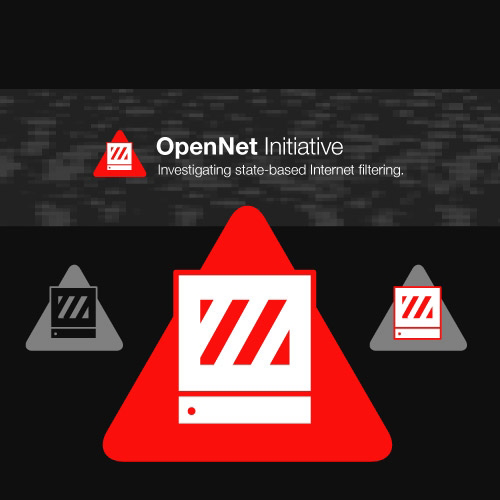
\includegraphics[width=0.3\textwidth]{oni.png}
  \label{fig:ejemplo}
\end{figure}
}

\frame
{
\transdissolve[duration=0.2]
\frametitle{El prop\'osito de la ONI}
Mediante el empleo de un enfoque multidiciplinario, la ONI se encarga de investigar, analizar y exponer las pr\'acticas de filtrado y vigilancia en Internet, de una manera cre\'ible y sustentable. Teniendo como intenci\'on descubrir los peligros y las consecuencias potenciales de estas pr\'acticas de censura y filtrado.
\begin{figure}
  \centering
    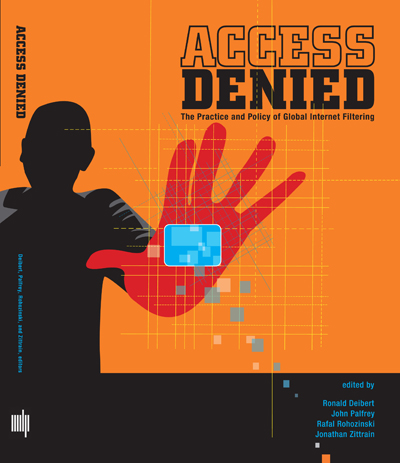
\includegraphics[width=0.35\textwidth]{img.jpg}
  \label{fig:ejemplo}
\end{figure}
}


\section{Filtrado en Internet}
\subsection{Enfoques de Filtrado}
\frame
{
\transdissolve[duration=0.2]
\frametitle{La censura de Internet}
Practica 
}

\subsection{Puntos de Control}
\frame
{
\transdissolve[duration=0.2]
\frametitle{Filtrado en la Red}
Practica 
}


\end{document}
